\documentclass{ximera}

 

\usepackage{epsfig}

\graphicspath{
  {./}
  {figures/}
}

\usepackage{morewrites}
\makeatletter
\newcommand\subfile[1]{%
\renewcommand{\input}[1]{}%
\begingroup\skip@preamble\otherinput{#1}\endgroup\par\vspace{\topsep}
\let\input\otherinput}
\makeatother

\newcommand{\includeexercises}{\directlua{dofile("/home/jim/linearAlgebra/laode/exercises.lua")}}

%\newcounter{ccounter}
%\setcounter{ccounter}{1}
%\newcommand{\Chapter}[1]{\setcounter{chapter}{\arabic{ccounter}}\chapter{#1}\addtocounter{ccounter}{1}}

%\newcommand{\section}[1]{\section{#1}\setcounter{thm}{0}\setcounter{equation}{0}}

%\renewcommand{\theequation}{\arabic{chapter}.\arabic{section}.\arabic{equation}}
%\renewcommand{\thefigure}{\arabic{chapter}.\arabic{figure}}
%\renewcommand{\thetable}{\arabic{chapter}.\arabic{table}}

%\newcommand{\Sec}[2]{\section{#1}\markright{\arabic{ccounter}.\arabic{section}.#2}\setcounter{equation}{0}\setcounter{thm}{0}\setcounter{figure}{0}}

\newcommand{\Sec}[2]{\section{#1}}

\setcounter{secnumdepth}{2}
%\setcounter{secnumdepth}{1} 

%\newcounter{THM}
%\renewcommand{\theTHM}{\arabic{chapter}.\arabic{section}}

\newcommand{\trademark}{{R\!\!\!\!\!\bigcirc}}
%\newtheorem{exercise}{}

\newcommand{\dfield}{{\sf dfield9}}
\newcommand{\pplane}{{\sf pplane9}}

\newcommand{\EXER}{\section*{Exercises}}%\vspace*{0.2in}\hrule\small\setcounter{exercise}{0}}
\newcommand{\CEXER}{}%\vspace{0.08in}\begin{center}Computer Exercises\end{center}}
\newcommand{\TEXER}{} %\vspace{0.08in}\begin{center}Hand Exercises\end{center}}
\newcommand{\AEXER}{} %\vspace{0.08in}\begin{center}Hand Exercises\end{center}}

% BADBAD: \newcommand{\Bbb}{\bf}

\newcommand{\R}{\mbox{$\Bbb{R}$}}
\newcommand{\C}{\mbox{$\Bbb{C}$}}
\newcommand{\Z}{\mbox{$\Bbb{Z}$}}
\newcommand{\N}{\mbox{$\Bbb{N}$}}
\newcommand{\D}{\mbox{{\bf D}}}
\usepackage{amssymb}
%\newcommand{\qed}{\hfill\mbox{\raggedright$\square$} \vspace{1ex}}
%\newcommand{\proof}{\noindent {\bf Proof:} \hspace{0.1in}}

\newcommand{\setmin}{\;\mbox{--}\;}
\newcommand{\Matlab}{{M\small{AT\-LAB}} }
\newcommand{\Matlabp}{{M\small{AT\-LAB}}}
\newcommand{\computer}{\Matlab Instructions}
\newcommand{\half}{\mbox{$\frac{1}{2}$}}
\newcommand{\compose}{\raisebox{.15ex}{\mbox{{\scriptsize$\circ$}}}}
\newcommand{\AND}{\quad\mbox{and}\quad}
\newcommand{\vect}[2]{\left(\begin{array}{c} #1_1 \\ \vdots \\
 #1_{#2}\end{array}\right)}
\newcommand{\mattwo}[4]{\left(\begin{array}{rr} #1 & #2\\ #3
&#4\end{array}\right)}
\newcommand{\mattwoc}[4]{\left(\begin{array}{cc} #1 & #2\\ #3
&#4\end{array}\right)}
\newcommand{\vectwo}[2]{\left(\begin{array}{r} #1 \\ #2\end{array}\right)}
\newcommand{\vectwoc}[2]{\left(\begin{array}{c} #1 \\ #2\end{array}\right)}

\newcommand{\ignore}[1]{}


\newcommand{\inv}{^{-1}}
\newcommand{\CC}{{\cal C}}
\newcommand{\CCone}{\CC^1}
\newcommand{\Span}{{\rm span}}
\newcommand{\rank}{{\rm rank}}
\newcommand{\trace}{{\rm tr}}
\newcommand{\RE}{{\rm Re}}
\newcommand{\IM}{{\rm Im}}
\newcommand{\nulls}{{\rm null\;space}}

\newcommand{\dps}{\displaystyle}
\newcommand{\arraystart}{\renewcommand{\arraystretch}{1.8}}
\newcommand{\arrayfinish}{\renewcommand{\arraystretch}{1.2}}
\newcommand{\Start}[1]{\vspace{0.08in}\noindent {\bf Section~\ref{#1}}}
\newcommand{\exer}[1]{\noindent {\bf \ref{#1}}}
\newcommand{\ans}{}
\newcommand{\matthree}[9]{\left(\begin{array}{rrr} #1 & #2 & #3 \\ #4 & #5 & #6
\\ #7 & #8 & #9\end{array}\right)}
\newcommand{\cvectwo}[2]{\left(\begin{array}{c} #1 \\ #2\end{array}\right)}
\newcommand{\cmatthree}[9]{\left(\begin{array}{ccc} #1 & #2 & #3 \\ #4 & #5 &
#6 \\ #7 & #8 & #9\end{array}\right)}
\newcommand{\vecthree}[3]{\left(\begin{array}{r} #1 \\ #2 \\
#3\end{array}\right)}
\newcommand{\cvecthree}[3]{\left(\begin{array}{c} #1 \\ #2 \\
#3\end{array}\right)}
\newcommand{\cmattwo}[4]{\left(\begin{array}{cc} #1 & #2\\ #3
&#4\end{array}\right)}

\newcommand{\Matrix}[1]{\ensuremath{\left(\begin{array}{rrrrrrrrrrrrrrrrrr} #1 \end{array}\right)}}

\newcommand{\Matrixc}[1]{\ensuremath{\left(\begin{array}{cccccccccccc} #1 \end{array}\right)}}



\renewcommand{\labelenumi}{\theenumi)}
\newenvironment{enumeratea}%
{\begingroup
 \renewcommand{\theenumi}{\alph{enumi}}
 \renewcommand{\labelenumi}{(\theenumi)}
 \begin{enumerate}}
 {\end{enumerate}\endgroup}



\newcounter{help}
\renewcommand{\thehelp}{\thesection.\arabic{equation}}

%\newenvironment{equation*}%
%{\renewcommand\endequation{\eqno (\theequation)* $$}%
%   \begin{equation}}%
%   {\end{equation}\renewcommand\endequation{\eqno \@eqnnum
%$$\global\@ignoretrue}}

%\input{psfig.tex}

\author{Martin Golubitsky and Michael Dellnitz}

%\newenvironment{matlabEquation}%
%{\renewcommand\endequation{\eqno (\theequation*) $$}%
%   \begin{equation}}%
%   {\end{equation}\renewcommand\endequation{\eqno \@eqnnum
% $$\global\@ignoretrue}}

\newcommand{\soln}{\textbf{Solution:} }
\newcommand{\exercap}[1]{\centerline{Figure~\ref{#1}}}
\newcommand{\exercaptwo}[1]{\centerline{Figure~\ref{#1}a\hspace{2.1in}
Figure~\ref{#1}b}}
\newcommand{\exercapthree}[1]{\centerline{Figure~\ref{#1}a\hspace{1.2in}
Figure~\ref{#1}b\hspace{1.2in}Figure~\ref{#1}c}}
\newcommand{\para}{\hspace{0.4in}}

\renewenvironment{solution}{\suppress}{\endsuppress}

\ifxake
\newenvironment{matlabEquation}{\begin{equation}}{\end{equation}}
\else
\newenvironment{matlabEquation}%
{\let\oldtheequation\theequation\renewcommand{\theequation}{\oldtheequation*}\begin{equation}}%
  {\end{equation}\let\theequation\oldtheequation}
\fi

\makeatother


\title{mo16.tex}

\begin{document}
\begin{abstract}
BADBAD
\end{abstract}
\maketitle

\chapter{Laplace Transforms}

\subsection*{Section~\protect{\ref{S:13.1}} The Method of Laplace Transforms}
\rhead{S:13.1}{THE METHOD OF LAPLACE TRANSFORMS}

\exer{c13.1.0a} \ans ${\cal L}[e^{3t}-2e^{-4t}](s) = \frac{1}{s-3} -
\frac{2}{s+4}$.

\exer{Ex:pf} $\dps\frac{a_1}{s-r_1} + \frac{a_2}{s-r_2} = 
\frac{a_1(s-r_2)+a_2(s-r_1)}{(s-r_1)(s-r_2)} =
\frac{(a_1+a_2)s - (a_1r_2+a_2r_1)}{(s-r_1)(s-r_2)}$.

\exer{c13.1.0B} \ans $\dps x(t) = 4e^{-3t}-3e^{-2t}$.

\soln $\dps\frac{s-1}{s^2+5s+6} = \frac{s-1}{(s+3)(s+2)} =
\frac{4}{s+3} - \frac{3}{s+2}$.

\exer{c13.1.1a} \ans The solution to the initial value problem is
$\dps x(t) = -\frac{1}{5}(e^{4t}+9e^{-t})$.

\soln Using properties~\Ref{Tprops}(a,c), compute:
\[
\begin{array}{rcl}
0 & = & {\cal L}[\ddot{x} - 3\dot{x} - 4x] \\
& = & (s^2{\cal L}[x] - sx(0) - \dot{x}(0)) - 3(s{\cal L}[x] - x(0))
- 4{\cal L}[x] \\
& = & (s^2 - 3s - 4){\cal L}[x] + (3 - s)x(0) - \dot{x}(0) \\
& = & (s^2 - 3s - 4){\cal L}[x] + 7 - 2s.
\end{array}
\]
Simplify to obtain
\[
{\cal L}[x] = \frac{7-2s}{(s-4)(s+1)} = 
-\frac{1}{5}\left(\frac{1}{s-4} + \frac{9}{s+1}\right).
\]
So, using \Ref{eq:Lexp},
${\cal L}[x] = {\cal L}[-\frac{1}{5}(e^{4t}+9e^{-t})]$.  By property 
\Ref{Tprops}(b), ${\cal L}^{-1}$ exists, so we can compute 
$x(t) = -\frac{1}{5}(e^{4t}+9e^{-t})$.

\exer{exer:kderLap} The case $k = 1$ is true by \Ref{Tprops}(c), that is
\[
{\cal L}\left[\frac{dy}{dt}\right] = s{\cal L}[y] = y(0).
\]
Now, suppose
\[
{\cal L}\left[\frac{d^ky}{dt^k}\right] = s^k{\cal L}[y] - s^{k - 1}y(0)
- \cdots - \frac{d^{k - 1}y}{dt^{k - 1}}(0).
\]
Then we can compute
\[
{\cal L}\left[\frac{d^{k + 1}y}{dt^{k + 1}}\right] =
s{\cal L}\left[\frac{d^ky}{dt^k}\right] - \frac{d^ky}{dt^k}(0)
= s^{k + 1}{\cal L}[y] - s^{k}y(0)
- \cdots - s\frac{d^{k - 1}y}{dt^{k - 1}}(0) - \frac{d^ky}{dt^k}(0).
\]
So the formula is valid by induction on $k \geq 1$.



\subsection*{Section~\protect{\ref{S:13.3}} Laplace Transforms and Their Computation}
\rhead{S:13.3}{LAPLACE TRANSFORMS AND THEIR COMPUTATION}

\exer{c13.3.1a} \ans
\[
{\cal L}[4\cos(t - 1)] =
4\left(\frac{s\cos(1) + \sin(1)}{s^2 + 1}\right).
\]
\soln Compute ${\cal L}[x]$ using trigonometric identities and
Table~\ref{tab:Laplist}:
\[
\begin{array}{rcl}
{\cal L}[4\cos(t - 1)]
& = & 4{\cal L}[\cos(t)\cos(1) + \sin(t)\sin(1)] \\
& = & \dps 4\left(\cos(1)\frac{s}{s^2 + 1} + \sin(1)\frac{1}{s^2 + 1}\right).
\end{array}
\]

\exer{c13.3.1c} \ans
\[
{\cal L}[(t - 3)^2] = \frac{9s^2 - 6s + 2}{s^3}.
\]
\soln Compute ${\cal L}[x]$ using Table~\ref{tab:Laplist}:
\[
{\cal L}[(t - 3)^2] = {\cal L}[t^2] - 6{\cal L}[t] + 9{\cal L}[1]
= \frac{2}{s^3} - 6\left(\frac{1}{s^2}\right) + 9\left(\frac{1}{s}
\right).
\]

\exer{c13.3.2} \ans The solution to the initial value problem is
\[
x(t) = 2e^{-t}\cos(2t) - 2e^{-t}\sin(2t).
\]
\soln First, apply the Laplace transform to both sides of the differential
equation:
\[
0 = {\cal L}[\ddot{x}] + 2{\cal L}[\dot{x}] + 5{\cal L}[x]
= (s^2 + 2s + 5){\cal L}[x] - (2s - 2).
\]
Next, solve for ${\cal L}[x]$.  The denominator of the partial fraction
has no real roots, so complete the square, obtaining
\[
{\cal L}[x]
= \frac{2s - 2}{s^2 + 2s + 5}
= 2\frac{s - 1}{(s + 1)^2 + 4}
= 2\frac{(s + 1) - 2}{(s + 1)^2 + 4}
= 2\frac{s + 1}{(s + 1)^2 + 4} - 2\frac{2}{(s + 1)^2 + 4}.
\]
Now, let
\[
Y(s) = 2\frac{s}{s^2 + 4} - 2\frac{2}{s^2 + 4}.
\]
Then, using Table~\ref{tab:Laplist},
\[
{\cal L}^{-1}[Y(s)] = 2\cos(2t) - 2\sin(2t)
\]
and, by Proposition~\ref{prop:eHcLap1}(b),
\[
x(t) = {\cal L}^{-1}[Y(s + 1)] = e^{-1}{\cal L}^{-1}[Y(s)].
\]

\exer{c13.4.3b} \ans The solution to the initial value problem is
\[
x(t) = \frac{1}{13}\left(1 + e^{3t}\cos(2t) - 8e^{3t}\sin(2t)\right).
\]
\soln First, apply the Laplace transform to both sides of the differential
equation:
\[
\frac{1}{s} = {\cal L}[1]
= {\cal L}[\ddot{x}] - 6{\cal L}[\dot{x}] + 13{\cal L}[x]
= (s^2 - 6s + 13){\cal L}[x] - 1.
\]
Next, solve for ${\cal L}[x]$ by using partial fractions, then completing
the square:
\[
\begin{array}{rcl}
{\cal L}[x] & = & \frac{s + 1}{s(s^2 - 6s + 13)} \\
& = & \frac{1}{13}\left(\frac{1}{s}\right) +
\frac{1}{13}\left(\frac{s - 19}{s^2 - 6s + 13}\right) \\
& = & \frac{1}{13}\left(\frac{1}{s} +
\frac{s - 3}{(s + 3)^2 + 4} - 8\frac{2}{(s - 3)^2 + 4}\right).
\end{array}
\]
Now, let
\[
Y(s) = \frac{s}{s^2 + 4} - 8\frac{2}{s^2 + 4}.
\]
Then, using Table~\ref{tab:Laplist},
\[
{\cal L}^{-1}[Y(s)] = \cos(2t) - 8\sin(2t)
\]
and, by Proposition~\ref{prop:eHcLap1}(b),
\[
x(t) = \frac{1}{13}\left({\cal L}^{-1}\left[\frac{1}{s}\right] +
{\cal L}^{-1}[Y(s - 3)]\right) =
\frac{1}{13}\left(1 + e^{3t}{\cal L}^{-1}[Y(s)]\right).
\]

\exer{c13.2.2} \ans The solution to the initial value problem is
$x(t) = \frac{1}{30}(35e^{2t}-6e^t+e^{-4t})$.

\soln Apply the Laplace transform to both sides of the ordinary
differential equation:
\[
\frac{1}{s-1} = {\cal L}[e^t]
= {\cal L}[\ddot{x}] + 2{\cal L}[\dot{x}] - 8{\cal L}[x]
= (s^2 + 2s - 8){\cal L}[x] - (s + 4).
\]
Then, use partial fractions to solve for ${\cal L}[x]$, obtaining
\[
{\cal L}[x] = \frac{s+4}{(s + 4)(s - 2)}
= \frac{1}{s-2} + \frac{1}{(s-1)(s-2)(s+4)}
= \frac{1}{30}\left(\frac{35}{s-2} - \frac{6}{s-1} + \frac{1}{s-4}\right).
\]
Therefore, $x(t)=\frac{1}{30}(35e^{2t}-6e^t+e^{-4t})$.



\newpage
\subsection*{Section~\protect{\ref{S:PF}} Partial Fractions}
\rhead{S:PF}{PARTIAL FRACTIONS}

\exer{c13.1.0C} \ans $e^{2t}+\frac{2}{3}e^{-3t}-\frac{5}{3}$.

\soln $Y(s)=\dps\frac{10}{s^3+s^2-6s} = \frac{10}{s(s-2)(s+3)}=
\frac{1}{s-2}-\frac{5/3}{s}+\frac{2/3}{s+3}$.  

Therefore,
${\cal L}\inv[Y(s)] = e^{2t}-\frac{5}{3}+\frac{2}{3}e^{-3t}$.

\exer{c13.3.3a} \ans
\[
\frac{2(s - 1)}{s^2 - 3s + 2} = \frac{2}{s - 2}.
\]
\soln To find the expansion into partial fractions using \Matlabp, type
\begin{verbatim}
p = [2 -2];
q = [1 -3 2];
[c,r] = residue(p,q)
\end{verbatim}
\Matlab returns the roots of the expansion as $r = (2,1)^t$ and
the corresponding scalars as $c = (2,0)^t$.

\exer{c13.3.3c} \ans
\[
\frac{3(s - 1)}{s^3 - s^1 + 4s - 4} = \frac{-\frac{3}{4}i}{s - 2i}
+ \frac{\frac{3}{4}i}{s + 2i}.
\]
\soln To find the expansion into partial fractions using \Matlabp, type
\begin{verbatim}
p = [3 -3];
q = [1 -1 4 -4];
[c,r] = residue(p,q)
\end{verbatim}
\Matlab returns the roots of the expansion as $r = (2i,-2i,1)^t$ and
the corresponding scalars as $c = (-\frac{3}{4}i,\frac{3}{4}i,0)^t$.

\exer{c13.3.4b}
\ans
\[
\frac{s^3 - 4s^2 + s + 6}{s^2 - 3s + 2}
= \frac{-4}{s - 1} + s - 1.
\]
\soln To find the expansion into partial fractions using \Matlabp, type
\begin{verbatim}
p = [1 -4 1 6];
q = [1 -3 2];
[c,r,k] = residue(p,q)
\end{verbatim}
\Matlab returns the roots of the expansion as $r = (2,1)^t$, the
corresponding scalars as $c = (0,-4)^t$, and the coefficients of the
polynomial term as $k = (1,-1)$.



\subsection*{Section~\protect{\ref{S:13.4}} Discontinuous Forcing}
\rhead{S:13.4}{DISCONTINUOUS FORCING}

\exer{Ex:cont} Verify that the equality holds by substituting $z(t)$ into
both sides:
\[
\begin{array}{rcl}
\dps \lim_{t \rightarrow 1^{+}}z(t) & = &
\dps \lim_{t \rightarrow 1^{+}}(1 - \cos(2(t - 1))) = 1 - \cos(0) = 0. \\
\dps \lim_{t \rightarrow 1^{-}}z(t) & = &
\dps \lim_{t \rightarrow 1^{-}}(0) = 0.
\end{array}
\]
So $z(t)$ is continuous.  Similarly, verify that $z(t)$ is differentiable
by substituting $z(t)$ into both sides of the equation, then using
L'H\^{o}spital's rule:
\[
\begin{array}{rcl}
\dps \lim_{h \rightarrow 0^{+}}\frac{z(1 + h) - z(1)}{h}
& = & \dps \lim_{h \rightarrow 0^{+}}\frac{(1 - \cos(2h)) - 0}{h}
= \dps \lim_{h \rightarrow 0^{+}}2\sin(2h) = 0. \\
\dps \lim_{h \rightarrow 0^{-}}\frac{z(1 + h) - z(1)}{h}
& = & \dps \lim_{h \rightarrow 0^{-}}\frac{0}{h} = 0.
\end{array}
\]

\exer{c13.4.5} \ans Figures~\ref{c13.4.5} show the {\tt ode45} solution
to \Ref{eq:lapendexam} with different tolerances.  When the system is
evaluated with higher tolerance, the Dirac delta function is evaluated
more accurately, since it is actually an impulse function.  Thus,
Figure~\ref{c13.4.5}c shows a behavioral change at $t = 1$, while the
other two figures do not.

\begin{figure}[htb]
                       \centerline{%
                       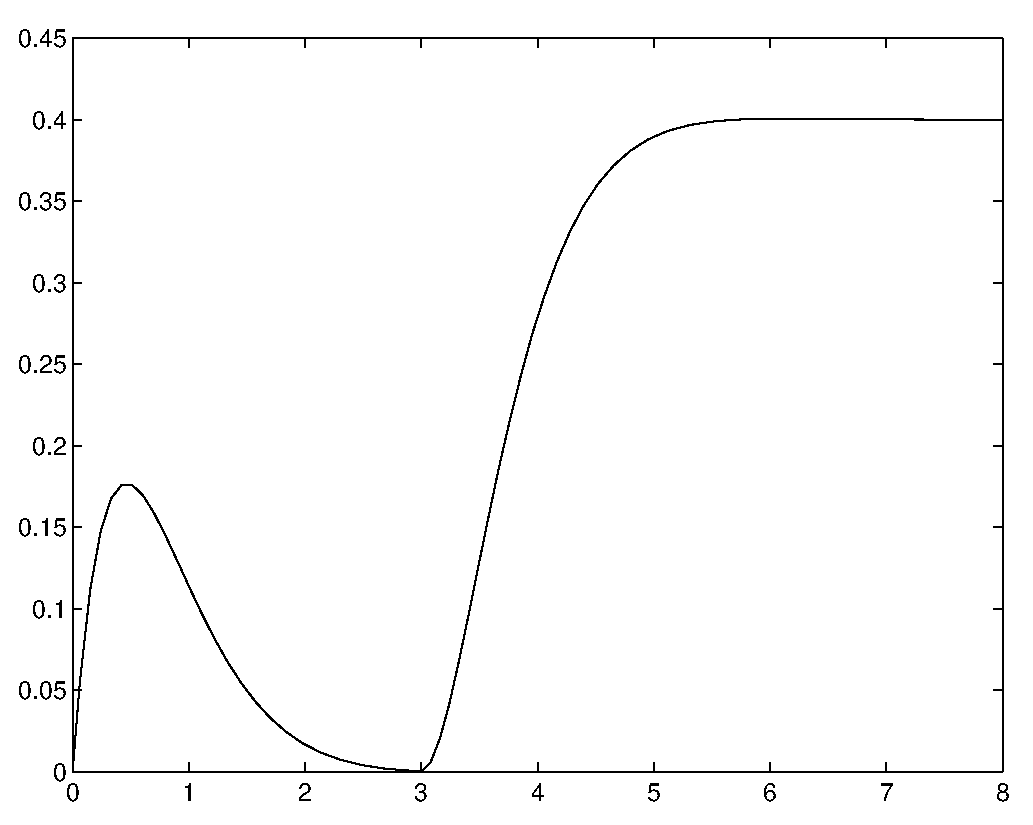
\psfig{file=exfigure/13-4-5a.eps,width=1.8in}
                       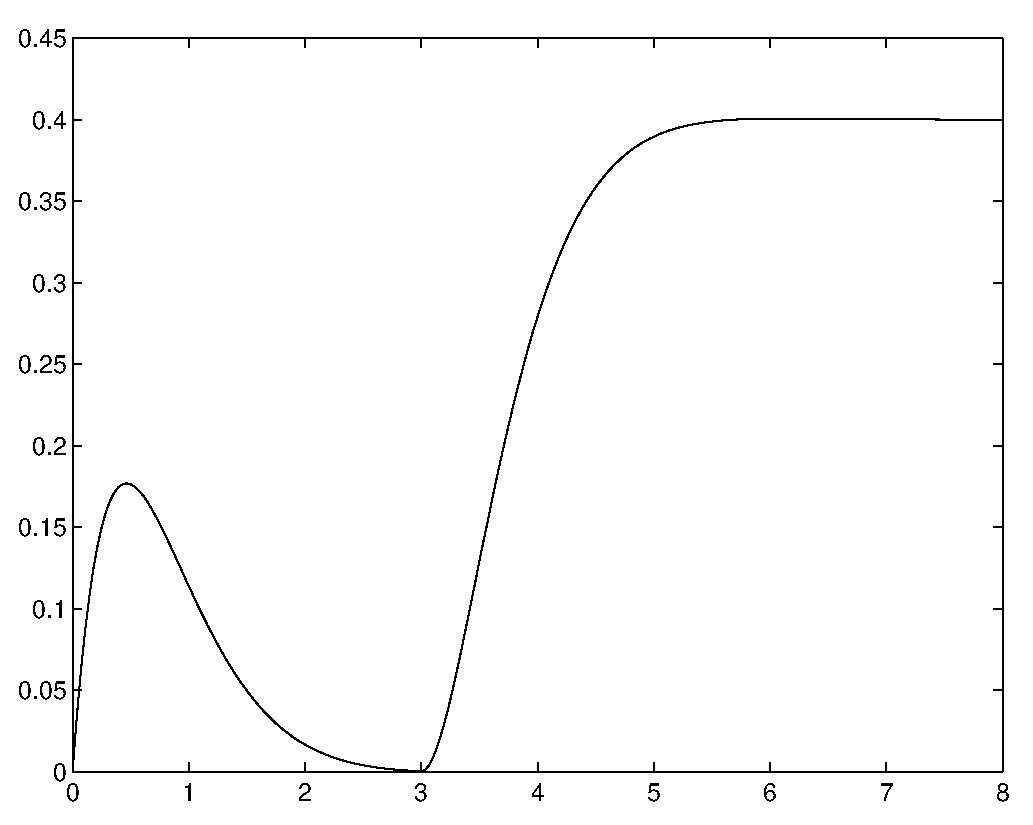
\psfig{file=exfigure/13-4-5b.eps,width=1.8in}
                       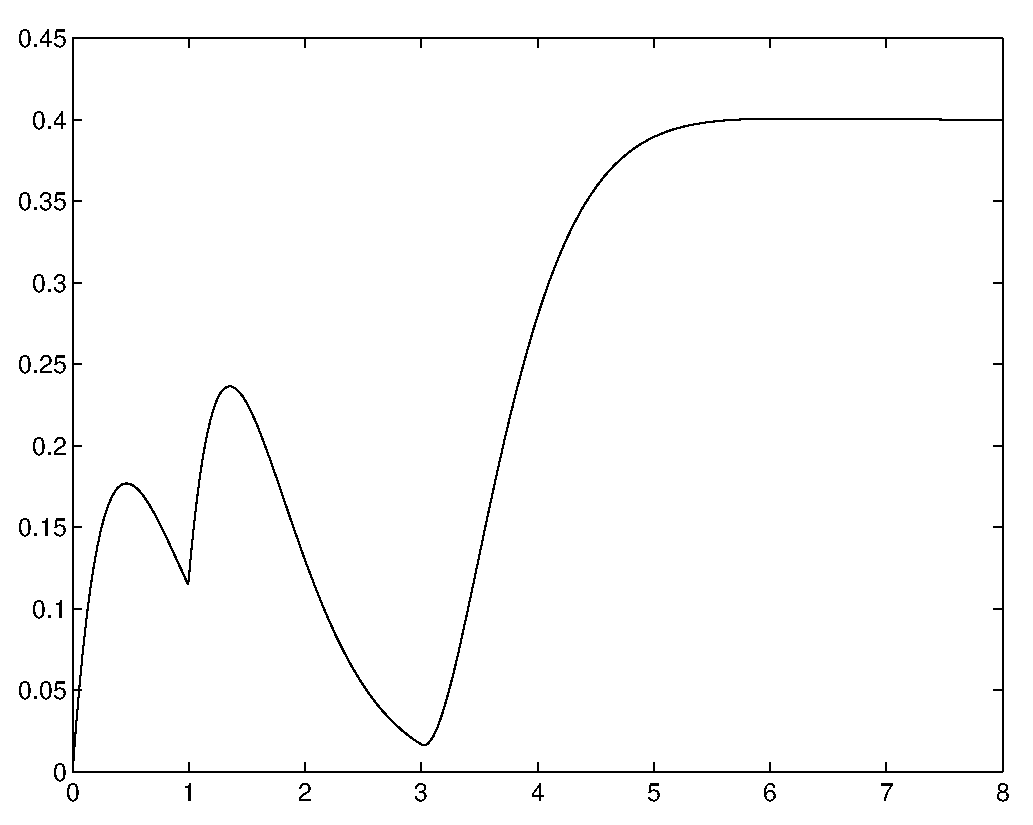
\psfig{file=exfigure/13-4-5c.eps,width=1.8in}}
                \centerline{{\tt eps = 1e-6}\hspace{1.2in}{\tt eps = 1e-8}
\hspace{1.2in}{\tt eps = 1e-10}}
		\exercapthree{c13.4.5}
\end{figure}

\end{document}
